\chapter{Introduction and Physics Background}
\section{The Standard Model: Theoretical framework}
The Standard Model of particle physics represents one of the most significant intellectual achievements in modern science.
%
Developed throughout the latter half of the $20^{th}$ century, it provides a quantum field theory framework that describes three of the four known fundamental forces—the electromagnetic, weak, and strong interactions---along with classifying all known elementary particles.
%
The mathematical formulation of the Standard Model is based on gauge theory, specifically quantum chromodynamics (QCD) and the electroweak theory, underpinned by the gauge symmetry group \(SU(3)\times SU(2)\times U(1)\).

The predictive power of the Standard Model has been repeatedly validated through precision experiments across multiple energy scales, from low-energy nuclear phenomena to the highest energy particle collisions achievable at modern accelerators.
%
Its crowning achievement came with the discovery of the Higgs boson in 2012 at the Large Hadron Collider (LHC), confirming the mechanism through which elementary particles acquire mass.
%
A schematic illustration of the standard model can be found in Fig.~\ref{fig:sm}

\begin{figure}
    \centering
    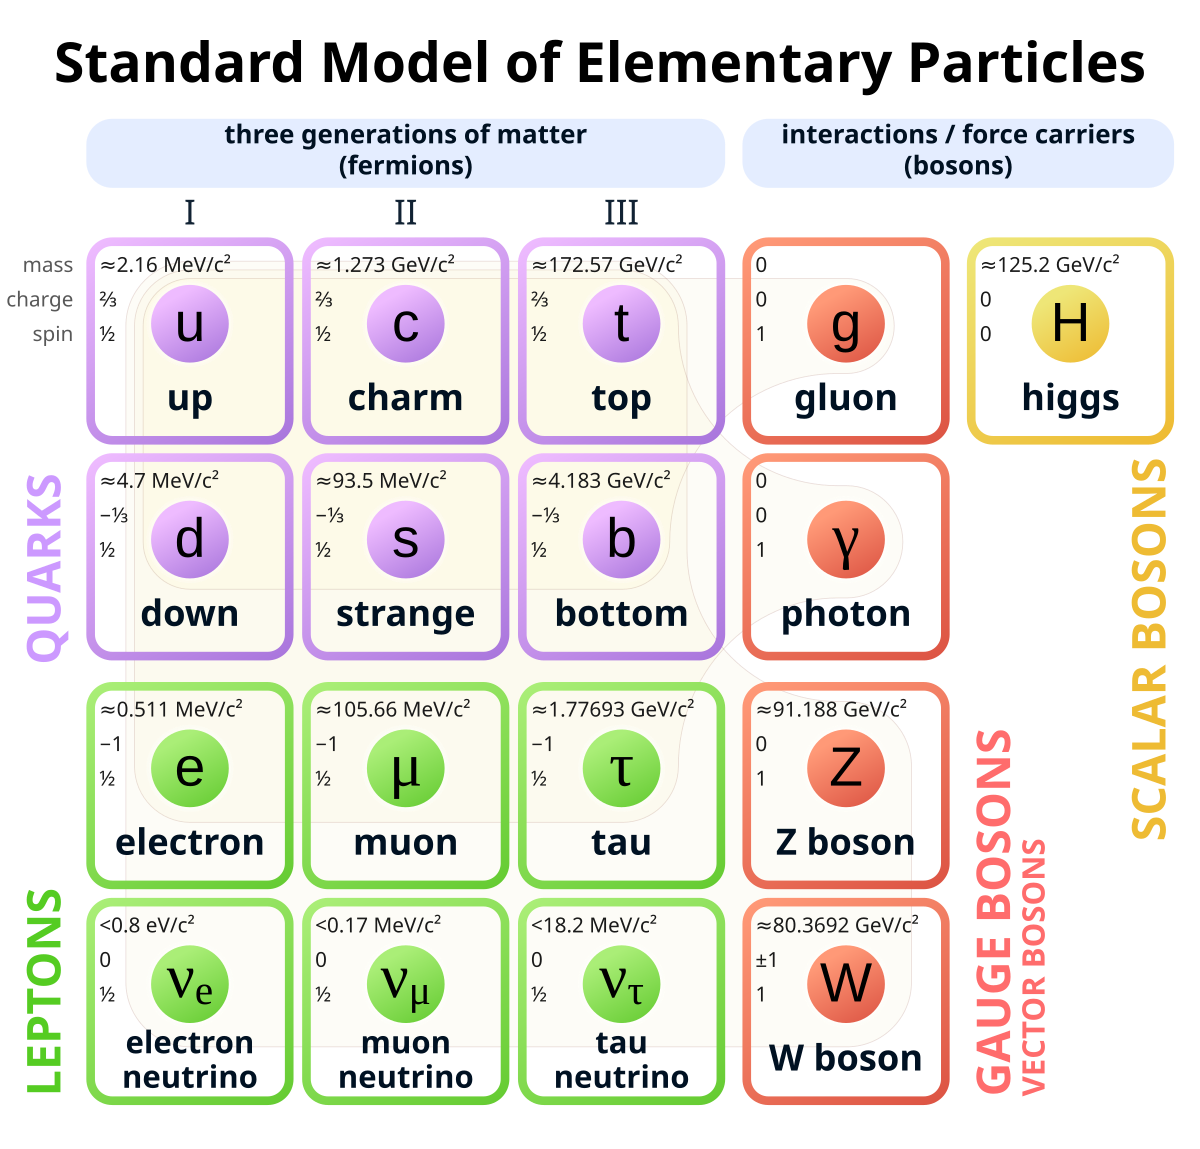
\includegraphics[width=0.5\linewidth]{figures/Standard_Model_of_Elementary_Particles.svg.png}
    \caption{A schematic illustration of the Standard Model.}
    \label{fig:sm}
\end{figure}
\subsection{Fundamental Particles and Forces}
The Standard Model categorizes elementary particles into two main families: fermions, which comprise matter, and bosons, which mediate forces between matter particles.
\subsubsection{Fermions: The Building Blocks of Matter}
Fermions, characterized by half-integer spin, obey the Pauli exclusion principle and are further classified into quarks and leptons, each arranged in three generations of increasing mass:
\paragraph{Quarks} (spin $ = \nicefrac{1}{2}$)
Quarks are catagorized into three generations as follows:
\begin{itemize}
    \item Up (u) and down (d),
    \item Charm (c) and strange (s),
    \item Top (t) and bottom (b).
\end{itemize}

Quarks carry fractional electric charge and color charge, and experience all fundamental forces.
%
They are confined within hadrons---composite particles categorized as baryons (three--quark states, like protons and neutrons) or mesons (quark--antiquark pairs).

\paragraph{Leptons} (spin $ = \nicefrac{1}{2}$)
Like quarks, leptons too are catagorized into three generations.
\begin{itemize}
    \item Electron (e) and electron neutrino ($\nu_e$),
    \item Muon $(\mu)$ and muon neutrino ($\nu_\mu$),
    \item Tau ($\tau$) and tau neutrino ($\nu_\tau$).
\end{itemize}

Electrons, muons, and taus carry unit electric charge and interact via electromagnetic and weak forces, while neutrinos are electrically neutral and interact only through the weak force, making them notoriously difficult to detect.

\subsubsection{Bosons: Force Carriers}
Bosons, with integer spin values, mediate the fundamental interactions. The Standard Model comprises the following bosons:
\begin{itemize}
    \item Photon $(\gamma)$: The massless spin--1 boson mediating the electromagnetic force,
    \item $W^\pm$ and $Z$ bosons: Massive spin--1 bosons mediating the weak force
    \item Gluons $(g)$: Eight massless spin-1 bosons mediating the strong force
    \item Higgs boson ($H$): A massive spin-0 boson associated with the Higgs field that gives mass to elementary particles
\end{itemize}

\subsection{Theoretical Framework and Symmetries}
The Standard Model is constructed through principles of quantum field theory where particles are excitations of underlying quantum fields.
%
Its mathematical structure is determined by local gauge invariance under the following specific symmetry transformations
\begin{itemize}
    \item $U(1)_Y$: Associated with weak hypercharge, the symmetry of electroweak theory
    \item $SU(2)_L$: Describes the weak isospin, acting on left-handed fermions
    \item $SU(3)_C$: Governs the strong interactions through color charge in QCD
\end{itemize}

Electroweak unification, demonstrated by Glashow, Weinberg, and Salam\kd{cite}, demonstrates how the electromagnetic and weak forces emerge as different aspects of a single electroweak interaction, which undergoes spontaneous symmetry breaking at low energies.

\subsection{The Higgs Mechanism and Mass Generation}
The Higgs mechanism, proposed by several physicists including Peter Higgs in the 1960s\kd{cite}, addresses the theoretical inconsistency of massive gauge bosons in a gauge-invariant theory.
%
The mechanism introduces a scalar field---the Higgs field---that permeates space and spontaneously breaks the electroweak symmetry when the universe cooled after the Big Bang.
%
This symmetry breaking generates masses for the W and Z bosons while leaving the photon massless, explaining the significant difference between the electromagnetic and weak forces at ordinary energies. Additionally, the Higgs field couples to fermions through Yukawa interactions\kd{cite}, generating their masses with coupling strengths proportional to the particle masses.

The discovery of the Higgs boson at the LHC in 2012, with properties consistent with Standard Model predictions, provided crucial experimental validation of this mechanism and completed the Standard Model's particle roster.

\subsection{Limitations and Beyond the Standard Model (BSM) Physics}
Despite its remarkable success, the Standard Model has several well-recognized limitations:

\begin{itemize}
\item It does not incorporate gravity, the fourth fundamental force.
\item It fails to explain the observed matter--antimatter asymmetry in the universe.
\item It does not account for dark matter or dark energy, which together constitute about 95\% of the universe's energy content.
\item  It requires fine-tuning of parameters, raising theoretical concerns like the hierarchy problem.
\item  It does not explain neutrino masses, which must exist given observed neutrino oscillations.
\end{itemize}
These limitations motivate theoretical extensions and experimental searches for physics beyond the Standard Model, including supersymmetry, grand unified theories, and various dark matter candidates.
%
Precision measurements at particle colliders provide one of the most powerful approaches to probe these potential extensions, making analysis techniques like those discussed in this thesis essential for advancing our fundamental understanding of nature.

\section{Fundamental role of cross section measurements in particle physics}

Differential cross section measurements are the fundamental currency of scientific exchange in particle physics, serving as the primary bridge between theoretical predictions and experimental observations.
%
These measurements quantify the probability density of specific particle interactions as a function of kinematic variables, providing the essential link between theoretical predictions and experimental observations.
%
 A cross section quantifies the probability of a specific particle interaction occurring and is typically expressed in units of area (barns, where $1$ barn $= 10^{-24} \mathrm{cm}^2$). This seemingly simple concept forms the cornerstone of how we test and validate our understanding of fundamental physics.
 
The Standard Model of particle physics---our most successful theory describing elementary particles and their interactions---makes precise predictions for cross sections that can be directly tested at collider experiments.
%
Any statistically significant deviation between measured cross sections and theoretical predictions may signal the presence of new physics beyond the Standard Model\kd{cite}.

Cross sections are particularly powerful because they encode the underlying quantum field theory structure in a form that can be directly probed by experiment.
%
For instance, measurements of jet production cross sections at different energy scales reveal the running of the strong coupling constant \(\alpha_S\)\kd{cite}, while precision electroweak cross section measurements constrain the properties of the Higgs boson and other fundamental particles\kd{cite}.
%
In searches for physics beyond the Standard Model, differential cross section measurements can reveal subtle deviations that point to new particles or interactions, even when direct observation is beyond experimental reach.

These measurements also serve a crucial role in constraining effective field theories (EFTs) that parameterize potential new physics in a model-independent way.
%
By measuring differential distributions with high precision, experiments can place bounds on EFT coefficients, narrowing the space of viable theoretical extensions to the Standard Model \kd{cite}.
%
The ongoing precision program at the Large Hadron Collider (LHC) relies heavily on refined cross section measurements to extract maximum physical insight from collected data.

\section{Cross Section Measurements: From Theory to Experiment}

The measurement of cross sections is a cornerstone of experimental particle physics, providing a direct link between theoretical predictions and observable phenomena. Cross sections quantify the likelihood of specific interactions or scattering processes between particles and are expressed in units of area, typically barns (\(1 \, \text{barn} = 10^{-28} \, \text{m}^2\)).

\subsection{Theory}

The cross section (\(\sigma\)) represents the effective area within which two particles must interact for a particular process to occur.
%
For collisions between discrete particles, the cross section is defined as the area transverse to their relative motion.
%
If the particles were to interact via contact forces (e.g., hard spheres), the cross section corresponds to their geometric size.
%
For long--range forces however, (e.g., electromagnetic or gravitational interactions), the cross section is larger than the physical dimensions of the particles due to action-at-a-distance effects.
%
The differential cross section (\(\frac{d\sigma}{d\Omega}\)) provides additional granularity by describing how the probability of scattering depends on specific final-state variables, such as scattering angle (\(\theta\)) or energy transfer. It is defined as:
\begin{equation}
    \frac{\dd\sigma}{\dd\Omega} = \frac{\text{Number of events scattered into } \dd\Omega}{\text{Incident flux} \times \text{Target density}}.
\end{equation}

The total cross section can be recovered by integrating over solid angle:
\begin{equation}
\sigma = \int_{4\pi} \frac{\dd\sigma}{\dd\Omega} \, \dd\Omega.
\end{equation}

Differential cross sections are have a long history of providing valuable insights for probing fundamental properties of particles and interactions.
%
For example, Rutherford scattering experiments revealed the existence of atomic nuclei by analyzing angular distributions of scattered alpha particles.\kd{cite}

\subsection{Experimental Measurement}

Experimentally, cross sections are determined by measuring the rate of particle interactions under controlled conditions. Consider a beam of incoming particles with flux \(J\) (\(s^{-1}\)) directed at a target slab with thickness \(\dd x\) and density \(n\).
%
The probability (\(\dd p\)) of scattering within this slab is proportional to the product of the target density, thickness, and cross section: \(\dd p = n \,\sigma\, \dd x\).

The rate of scattered particles (\(J_{\text{scattered}}\)) can then be expressed as:
\begin{align}
J_{\text{scattered}} &= J\times \sigma\times n\; \dd x.\\
\therefore \sigma &= \frac{J_{\text{scattered}}}{J\, n \, \dd x}.
\end{align}


Modern experiments employ arrays of detectors positioned at various angles around the interaction region to measure differential cross sections.
%
These detectors count scattered particles as a function of solid angle (\(d\Omega\)), enabling precise determination of angular distributions.
%
Normalization factors are critical for accurate measurements.
%
These include corrections for beam intensity fluctuations, detector efficiency, and background noise.
%
Additionally, advanced simulations are used to account for detector distortions and acceptance effects.

\subsection{Applications in Particle Physics}

Cross section measurements serve multiple roles in particle physics.
%
Comparing measured cross sections with predictions from quantum field theory validates and tests theoretical models like Quantum Chromodynamics (QCD) and electroweak theory.
%
Deviations from expected cross sections may indicate new phenomena, such as supersymmetric particles or dark matter candidates.
%
Differential cross sections also provide constraints on effective field theories and parton distribution functions (PDFs), essential for understanding the internal structure of hadrons.
%
Unfolded cross section measurements allow comparisons with theoretical models years after data collection, even if detector simulations are no longer available, further enhancing their utility, and future proofing the data.

Cross sections bridge theory and experiment by encapsulating interaction probabilities in a measurable form.
%
Their determination requires careful experimental design and analysis techniques to account for systematic uncertainties introduced by detector effects.






\section{Detector response in precision measurements}

The direct comparison between theoretical predictions and experimental measurements is fundamentally complicated by detector effects. Particle physics detectors are intricate technological marvels surrounding collision points, but they introduce distortions that must be carefully accounted for to extract the true physical distributions of interest. These detector effects include:

\begin{itemize}
\item \textbf{Finite resolution}: Detector components have limited precision in measuring particle energies, momenta, and positions.
\item \textbf{Acceptance effects}: Geometric constraints mean that some regions of phase space remain unobserved.
\item \textbf{Efficiency variations}: The probability of detecting particles varies across phase space and between particle types.
\item \textbf{Particle misidentification}: The detector may incorrectly classify particle types.
\item \textbf{Background contamination}: Processes other than the signal of interest contribute to the observed data.
\end{itemize}

The relationship between the true particle--level distribution (what we want to measure) and the detector--level distribution (what we actually observe) can be mathematically expressed as:

\begin{equation}
p_{\textrm{detector}}(x) = \int R(x|z)\;p_{\textrm{particle}}(z)\;\dd z
\end{equation}

Here, \(R(x | z)\) represents the detector response function that maps particle--level data \((Z)\) to detector--level data \(X\).
%
This function encapsulates all detector effects and is typically estimated using detailed simulation.\kd{cite}
%
The fundamental challenge of experimental particle physics is to invert this kernel to infer \(p(Z = z)\) from observed data \(p(X = x)\), a process known as unfolding or deconvolution \kd{cite}.

\section{Experimental challenges at modern colliders}

The Large Hadron Collider represents the energy and precision frontiers of particle physics, producing collision events of unprecedented complexity at energies up to 13 TeV.
%
Several experimental challenges at the LHC and other modern colliders make cross section measurements particularly demanding.

\begin{itemize}
\item \textbf{High--dimensional phase spaces}: Modern measurements often involve multiple correlated observables, creating high--dimensional distributions that are difficult to analyze with traditional methods.
\item \textbf{Limited statistics in extreme regions}: Rare processes or the tails of distributions often contain valuable physics information but suffer from limited statistics.
\item \textbf{Complex detector effects}: Detectors have non-trivial response functions that can vary significantly across phase space, and are only known implicitly through precision simulations. Their explicit functional form is unknown.
\item \textbf{Theoretical uncertainties}: Precision measurements are increasingly limited by theoretical uncertainties in both signal and background modeling.
\item \textbf{Computational constraints}: Detailed simulation of detector response requires substantial computing resources, limiting the statistical precision of response modeling.
\end{itemize}

These challenges make the unfolding problem increasingly difficult, particularly as measurements probe more complex final states and differential distributions.
%
For example, measurements of jet substructure, which probe the detailed radiation pattern within collimated sprays of particles, involve observables with complex correlations and detector effects that vary based on jet energy, rapidity, and substructure properties themselves. \kd{cite}

The need for unfolding arises from the fundamental requirement to present results in a detector--independent form that can be directly compared with theory predictions or results from different experiments. Without this correction, theoretical interpretations would need to incorporate experiment--specific detector simulations, significantly complicating scientific exchange and theoretical analysis.

\section{Thesis Scope and Physics Impact}

This dissertation focuses on developing, analyzing, and applying novel machine learning methods for cross section measurements in particle physics, with particular emphasis on unbinned approaches that overcome limitations of traditional techniques. The work spans the spectrum from improving binned methods with neural posterior estimation to completely binning-free approaches for both full distributions and statistical moments.

The primary contributions of this thesis include:

\begin{enumerate}
\item Development of Neural Posterior Unfolding (NPU), enhancing binned approaches through normalizing flows and amortized inference
\item Introduction of Moment Unfolding, directly deconvolving distribution moments without binning
\item Creation of Reweighting Adversarial Networks (RAN), a general framework for unbinned spectrum unfolding
\item Analysis of event correlations in unfolded data and their impact on uncertainty estimation
\item Investigation of symmetry discovery with SymmetryGAN and its connections to measurement constraints
\end{enumerate}

These methodological advances address fundamental challenges in experimental particle physics, potentially enhancing the precision and scope of measurements at the LHC and future colliders. Specific physics impacts include:

\begin{itemize}
\item Improved precision in jet substructure measurements, enabling better discrimination between different theoretical models of QCD radiation
\item Enhanced sensitivity to effective field theory parameters through direct moment unfolding
\item More robust uncertainty quantification in high-dimensional measurements
\item Computational efficiency gains allowing for more detailed systematic studies
\item Framework for incorporating detector response uncertainties in the unfolding process
\end{itemize}

By bridging sophisticated machine learning techniques with the specific requirements of particle physics measurements, this work aims to advance our ability to extract fundamental physical insights from complex experimental data. The methods developed here have applications beyond particle physics, potentially benefiting any field where deconvolution of instrumental effects is necessary for scientific interpretation.